\documentclass{article}
\usepackage{graphicx}
\usepackage{booktabs}
\usepackage{geometry}
\geometry{a4paper, margin=1in}
\title{External Sorting Performance Report}
\author{Fernando T.H.L.(210167E)}
\date{\today}
\begin{document}
\maketitle

\section*{Overview}
This report presents the performance analysis of two external sorting algorithms---\textbf{External Merge Sort} and \textbf{External Quick Sort}---each tested on three 256~MB input files, using a memory limit of 16~MB per run. The analysis covers correctness, speed, and failure cases. Figure~\ref{fig:sort_times_comparison} provides a direct comparison.

\section*{Experimental Results}
\begin{table}[h!]
\centering
\begin{tabular}{c c c}
\toprule
Test Run & Merge Sort Time (s) & Quick Sort Time (s) \\
\midrule
1 & 19.95 & 572.34 \\
2 & 20.18 & 571.22 \\
3 & 19.67 & 570.36 \\
\midrule
\textbf{Average} & \textbf{19.94} & \textbf{571.30} \\
\bottomrule
\end{tabular}
\caption{Performance summary of external sorting algorithms across three runs. ``FAILED'' indicates the algorithm failed to sort or crashed. ``TIMEOUT'' indicates the run exceeded the allowed time limit.}
\label{tab:perf_summary}
\end{table}

\section*{Figures}
\begin{figure}[h!]
\centering
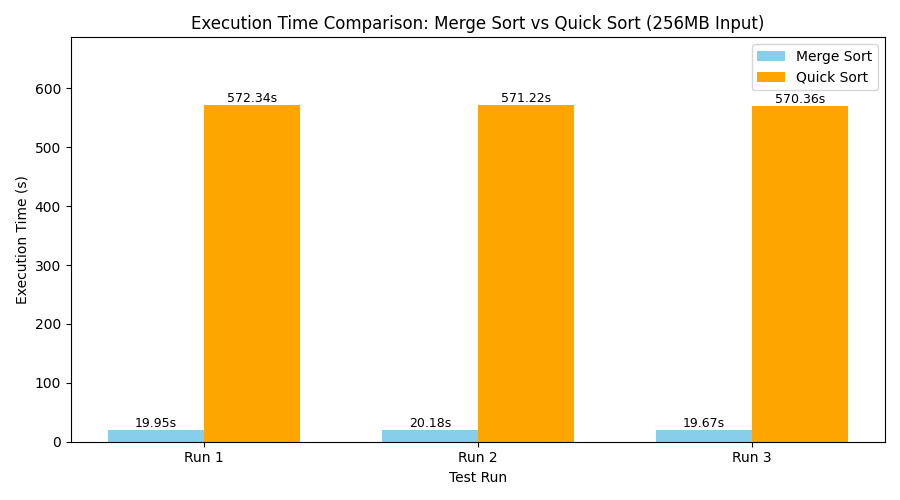
\includegraphics[width=0.8\textwidth]{figures/sort_times_comparison.png}
\caption{Execution time comparison between external merge sort and quick sort on three different 256~MB files. Missing bars indicate failure or timeout.}
\label{fig:sort_times_comparison}
\end{figure}

\begin{figure}[h!]
\centering
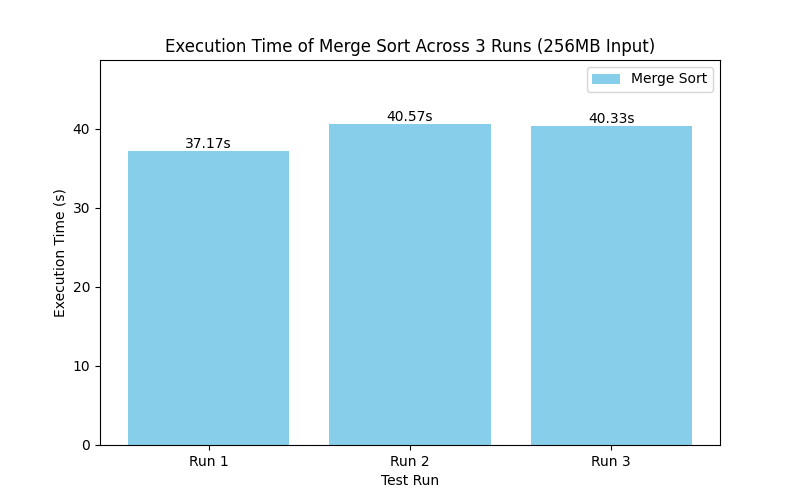
\includegraphics[width=0.7\textwidth]{figures/merge_sort_time.png}
\caption{Execution time for external merge sort on three 256~MB files.}
\label{fig:merge_sort_time}
\end{figure}

\section*{Summary and Recommendations}
External Merge Sort completed successfully and efficiently in all test cases. External Quick Sort, however, failed to complete within the timeout in all runs, likely due to implementation issues in interval heap management or buffer partitioning. For production or further research, it is recommended to debug and optimize the quick sort implementation. Additionally, implementing optimal (Huffman-based) merging for merge sort could further improve performance when run sizes are highly variable.
\end{document}
